\documentclass[10pt]{article}
\usepackage[paperwidth=215mm,paperheight=62mm,margin=2mm]{geometry}
\usepackage{fontspec}
\usepackage{tikz}
\usetikzlibrary{positioning}
\setmainfont{DejaVu Sans}
\pagestyle{empty}

\begin{document}
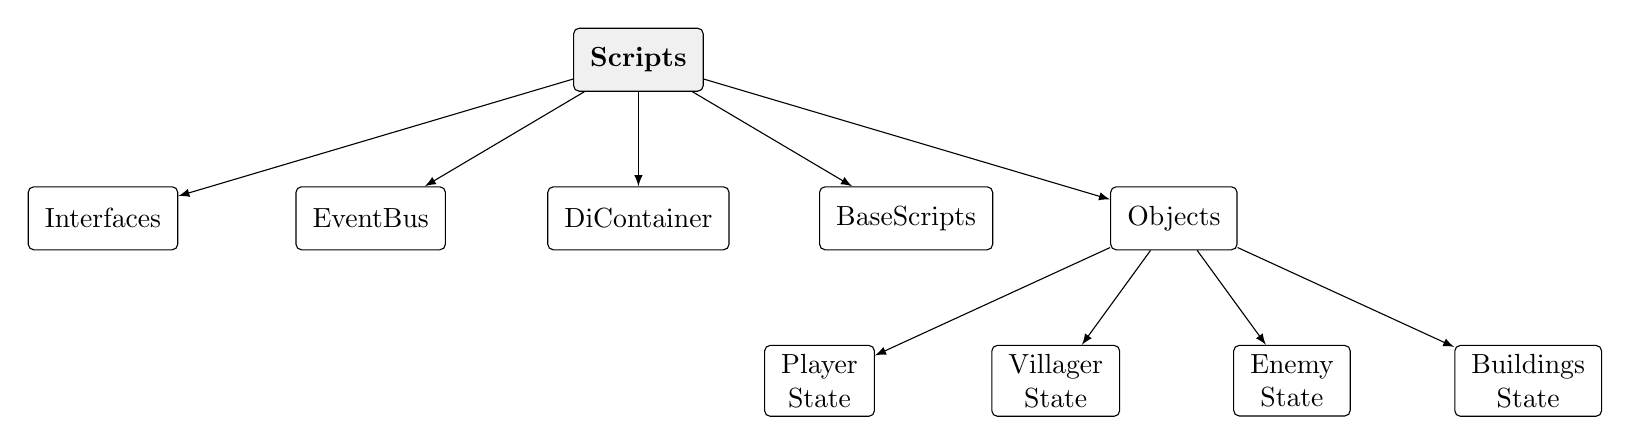
\begin{tikzpicture}[
  box/.style={
    draw,
    rounded corners=2pt,
    align=center,
    font=\normalsize,
    minimum height=8mm,
    inner xsep=6pt,
    fill=white
  },
  root/.style={box, fill=gray!12, font=\bfseries\normalsize},
  line/.style={draw, -latex}
]
\node[root] (scripts) {Scripts};
\node[box, below=12mm of scripts, xshift=-68mm] (interfaces) {Interfaces};
\node[box, below=12mm of scripts, xshift=-34mm] (eventbus) {EventBus};
\node[box, below=12mm of scripts] (dicontainer) {DiContainer};
\node[box, below=12mm of scripts, xshift=34mm] (base) {BaseScripts};
\node[box, below=12mm of scripts, xshift=68mm] (objects) {Objects};

\node[box, below=12mm of objects, xshift=-45mm] (player) {Player\\State};
\node[box, below=12mm of objects, xshift=-15mm] (villager) {Villager\\State};
\node[box, below=12mm of objects, xshift=15mm] (enemy) {Enemy\\State};
\node[box, below=12mm of objects, xshift=45mm] (buildings) {Buildings\\State};

\draw[line] (scripts) -- (interfaces);
\draw[line] (scripts) -- (eventbus);
\draw[line] (scripts) -- (dicontainer);
\draw[line] (scripts) -- (base);
\draw[line] (scripts) -- (objects);
\draw[line] (objects) -- (player);
\draw[line] (objects) -- (villager);
\draw[line] (objects) -- (enemy);
\draw[line] (objects) -- (buildings);
\end{tikzpicture}
\end{document}
